\section{Entwurf des zentralen Systems}\label{l:entwurf}

Im vorigen Abschnitt~\ref{l:konzeption}~(S.\pageref{l:konzeption}~ff.) wurde eine Anwendung konzipiert, die das gesamte Spektrum der Anforderungen abdeckt, die in den vorangegangenen Abschnitten beschrieben wurden. Der zentrale Bestandteil ist der Server, mit dem verschiedene GUIs über Schnittstellen kommunzieren. In diesem Abschnitt werden in Abschnitt~\ref{l:entwurf-server}~(S.\pageref{l:entwurf-server}) die wichtigsten Komponenten des Server beschrieben. Eine der wichtigsten GUIs, mit der alle Mitarbeiter arbeiten, ist das browserbasierte Interface, das in Abschnitt~\ref{l:entwurf-gui}~(S.\pageref{l:entwurf-gui}) beschrieben wird. Abschließend wird in Abschnitt~\ref{l:domänenmodell} das Domänenmodell vorgestellt, das allen Teilen der Anwendung zu grunde liegt.

\subsection{Server}\label{l:entwurf-server}

In Abbildung~\ref{chart:komponenten}~(S.\pageref{chart:komponenten}) finden sich die Komponenten des Servers grau eingefärbt.

\begin{figure}[htb]
\begin{center}
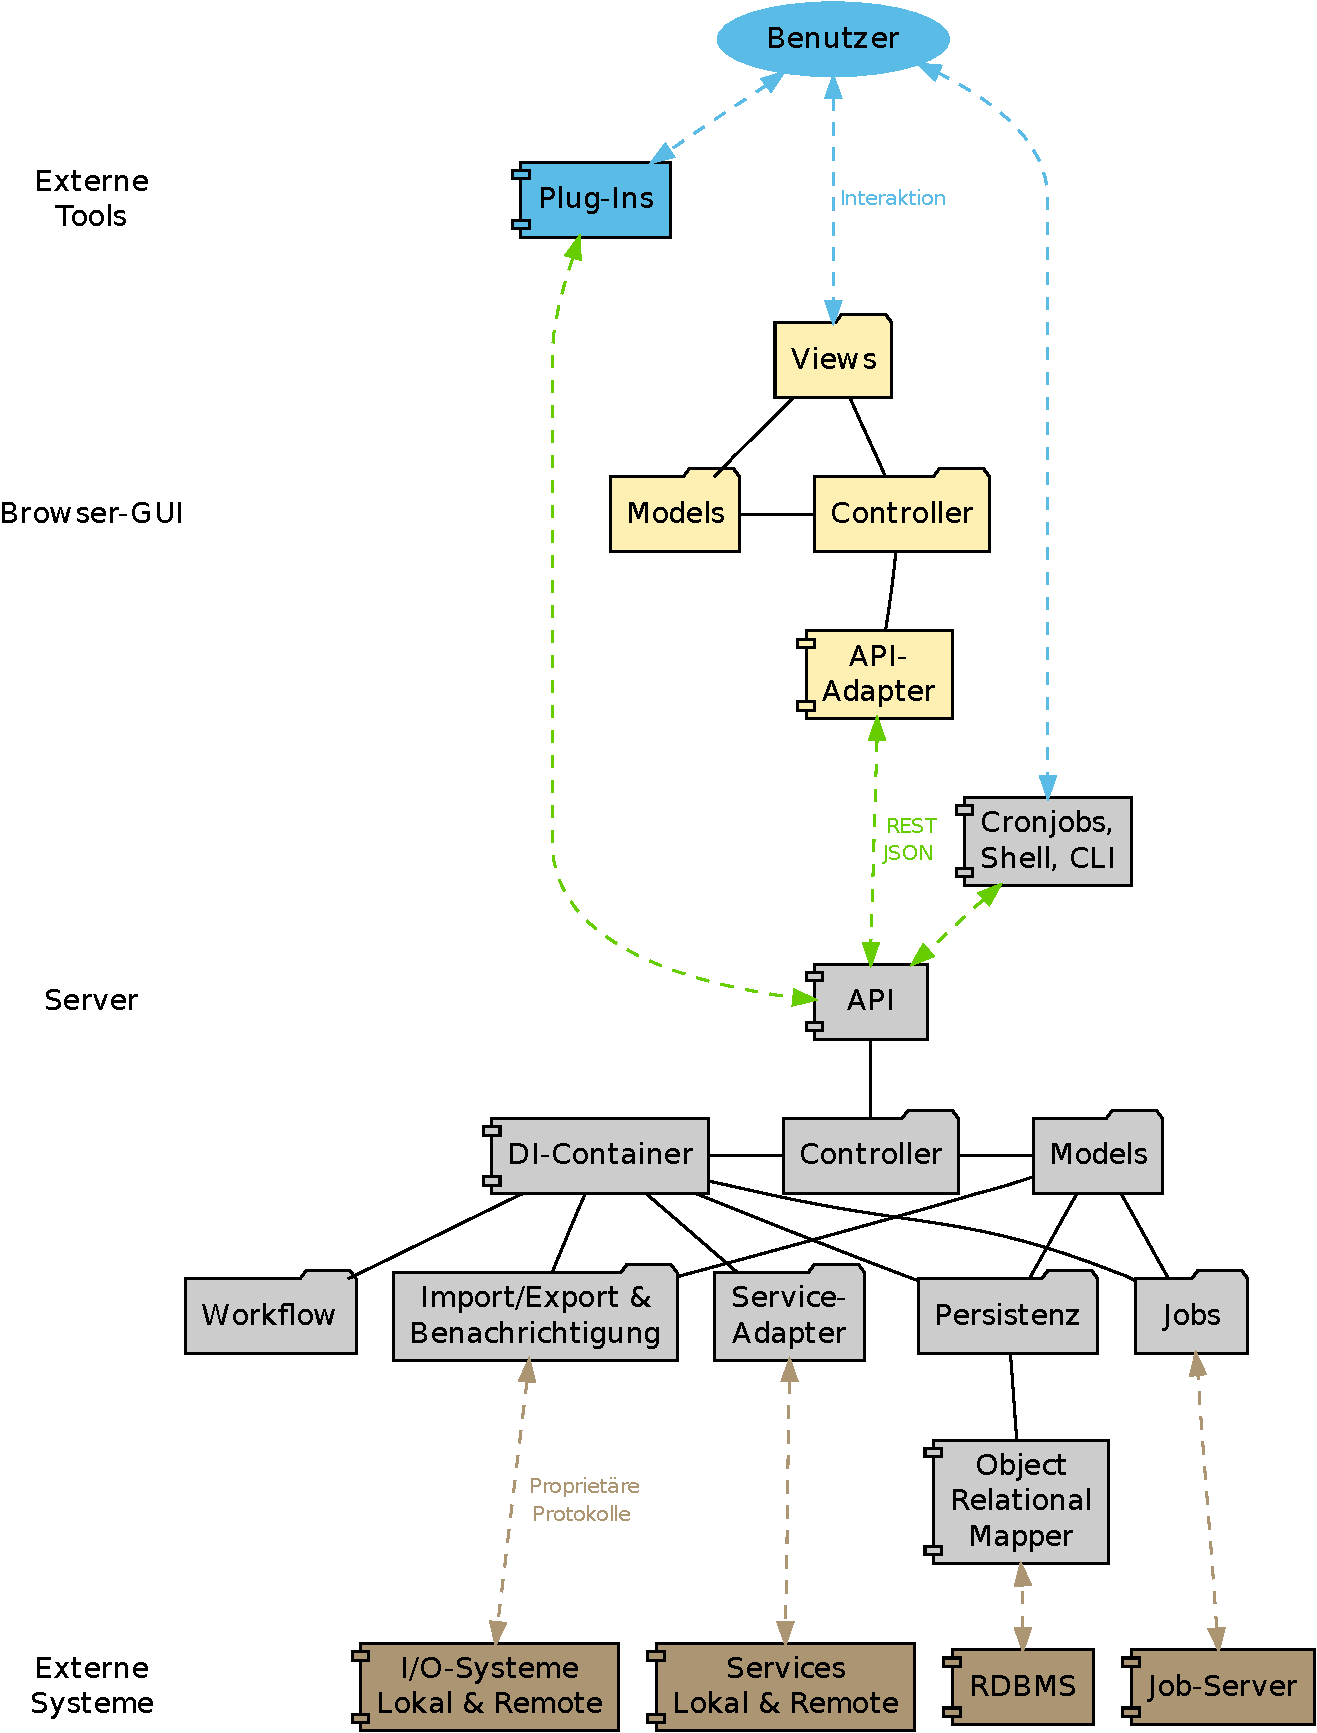
\includegraphics[width=0.7\textwidth]{media/komponenten.pdf}
\end{center}
\caption{Komponententen des zentralen Systems}
\label{chart:komponenten}
\end{figure}

\subsubsection{Core}

\subsubsection{Persistenz}

\subsubsection{Schnittstellen}

\subsubsection{Benachrichtigung}

\subsubsection{Pull-Export}

\subsubsection{Push-Export}

\subsection{Entwurf einer browserbasierten GUI}\label{l:entwurf-gui}

Diese vier Leitlinien repräsentieren die Grundgedanken bei der Entwicklung von der Anwendung:

\begin{itemize}
\item{Das wichtigste zuerst: Die aktuelle Aufgabe soll immer im Fokus der Darstellung liegen.}
\item{Schnell zum Ziel: Alle Aufgaben müssen leicht und umkompliziert durchführbar sein.}
\item{Nicht nerven: Ständige Benachrichtigungen lenken ab und müssen deswegen so gestaltet sein, dass diese sich nach den Präferenzen des Nutzers richten.}
\item{Hilfe nur einen Klick entfernt: Das Hilfesystem muss kontextsensitiv verfügbar sein und ist eine Kernfunktion der Anwendung}
\end{itemize}

Anforderungen, Grundsätze, Usability, Aufbau, Wireframes

Bei Kontroll-Aufgaben (Lektorat, QS) unterbrechungsfreies Arbeiten ermöglichen (Infinite-Scroll).

Die GUI muss deutlich einfacher zu bedienen sein, als z.B. Word oder Publishing-Systeme, sonst wird sie nicht von Kunden eingesetzt.

\subsubsection{Wireframes}

\subsection{Domänenmodell}\label{l:domänenmodell}

\begin{center}
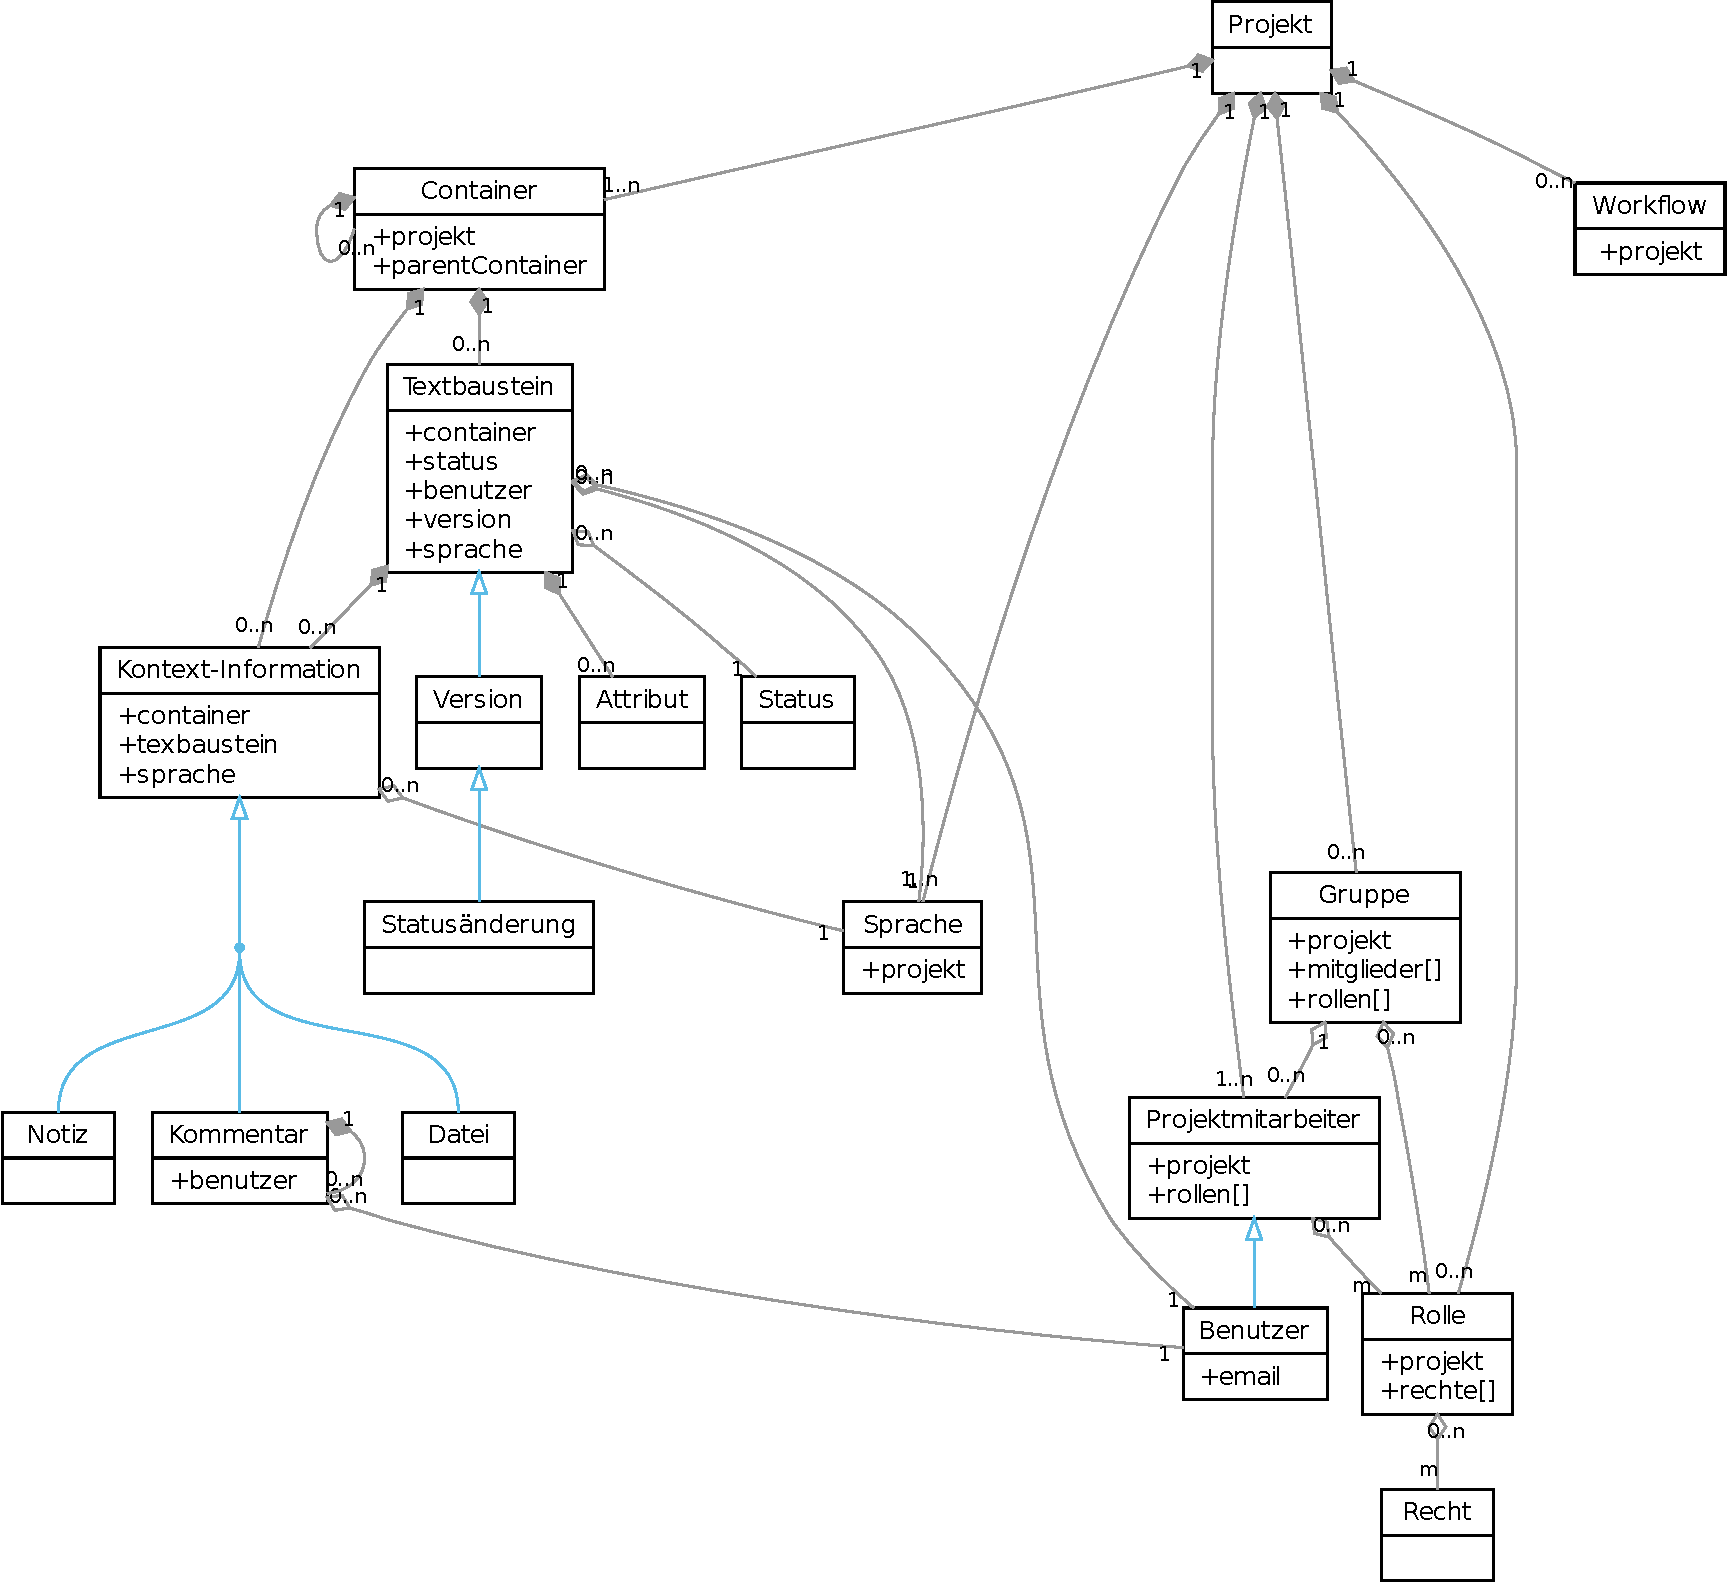
\includegraphics[width=\textwidth]{media/domain.pdf}
\captionof{figure}{Domänenmodell}\label{chart:domain}
\end{center}

Aus den vorangegangenen Überlegungen zur Anwendung und zum Workflow lässt sich ein Domänenmodell extrahieren, die einzelnen logischen Objekte innerhalb der Anwendung beschreibt, mit deren Hilfe alle Operationen abgebildet werden. Abbildung~\ref{chart:domain} zeigt das Modell in der Übersicht, dass die sich im Entwurf der Anwendung in deren Implementierung im Prototypen widerspiegelt.

\textsf{\textbf{Attribut}}\\Beschreibt die Attribute eines Textbausteins.

\textsf{\textbf{Benutzer}}\\Repräsentiert einen Benutzer des Systems

\textsf{\textbf{Container}}\\Containern dienen zur hierarchischen Organisation der Texte innerhalb des Projektes. Containern können weitere Container und Texte enthalten. Eine Container ohne übergeordneten Container befindet sich auf der obersten Ebene. Es kann mehrere Containern auf der obersten Ebene geben.

\textsf{\textbf{Gruppe}}\\Mitarbeiter können in Gruppen zusammengefasst werden. Dies erleichtert die Konfiguration des Workflows und der Rechte.

\textsf{\textbf{Kommentare}}\\Kommentare enthalten Hinweise und Fragen zu einzelnen Texten und Texbausteinen.

\textsf{\textbf{Kontext-Information}}\\Projektspezifische Kontext-Informationen lassen sich hinterlegen und Textbausteinen und Containern zuordnen.

\textsf{\textbf{Projekt}}\\Projekte bildet den Rahmen für alle Texte eines einzelnen Produktes.

\textsf{\textbf{Projektmitarbeiter}}\\Gestattet einem Benutzer die Mitarbeit an einem Projekt und legt dabei fest, welche Rechte dem Benutzer für das Projekt zustehen.

\textsf{\textbf{Recht}}\\Beschreibt ein Recht, eine Operation auf einem Objekt auszuführen.

\textsf{\textbf{Rolle}}\\Beschreibt die verschiedenen Rollen innerhalb der Anwendung. Die Rechte der Rollen sind durch die Zuordnung von Benutzern zu Projekten durch den Projektmitarbeiter immer an das jeweilige Projekt gebunden.

\textsf{\textbf{Sprache}}\\Die Texte jedes Projekts liegen in einer oder mehreren Sprachen vor.

\textsf{\textbf{Status}}\\Beschreibt die verschiedenen Zustände eines Textbausteins (vgl. Abschnitt \ref{l:konzept-workflow-status} · S.\pageref{l:konzept-workflow-status}).

\begin{enumerate}\itemsep -5pt
\item \texttt{Neu}, Textbaustein erzeugt
\item \texttt{Leer}, Textbaustein definiert
\item \texttt{Befüllt}, Textbaustein mit Inhalt befüllt
\item \texttt{Korrigiert}, Orthografie geprüft
\item \texttt{Geprüft}, Inhalt geprüft (Qualitätsicherung)
\item \texttt{Freigegeben}, durch Kunden freigegeben
\item \texttt{Veröffentlicht}, in Produkt übernommen
\end{enumerate}

\textsf{\textbf{Statusänderung}}\\Beschreibt eine Änderung eines Status durch einen Benutzer, z.B. durch Freigabe oder Überprüfung.

\textsf{\textbf{Textbaustein}}\\Beschreibt einen einzelnen Textbaustein.

\textsf{\textbf{Version}}\\Beschreibt eine Version des Inhalts eines Textbausteins.

\textsf{\textbf{Workflow}}\\Beschreibt einen projektspezifischen Workflow.
